\documentclass[openany, a4paper, 12pt]{report}
\usepackage[utf8]{inputenc}
\usepackage{color}
\usepackage{hyperref}
\usepackage{graphicx}
\usepackage{float}

\hypersetup {
	linkcolor = {black},
	urlcolor = {blue},
	menucolor = {black},
	colorlinks = true,
}

\begin{document}

	\begin{titlepage}
		\centering
		\vfill
		{
			\bfseries
			\vskip2cm
			\Large Università di Padova\\
			\vfill
			\Huge Artbit\\
			\Large Progetto per il corso di tecnologie web\\
			\vfill
			
			\begin{figure}[H]
				\centering
				
\includegraphics[width=0.6\linewidth]{logo.png}
			\end{figure}
			\large Davide Liu - 1140717 \\ Harwinder Singh - xxxxxxx \\ Pardeep Singh - xxxxxxx \\ Daniele Bianchin - xxxxxxx \\
			\vfill
			Sito web hostato all'indirizzo: \url{http://artbit.altervista.org/}\\
			{\small Credenziali per l'amministrazione:\\username: admin, password: admin\\}
			\vfill
			Indirizzo email del referente: davide.liu.@studenti.unipd.it\\
			\vfill
		}
	\end{titlepage}
	\pagenumbering{roman}
	\tableofcontents
	\newpage
	\pagenumbering{arabic}

	% Il progetto deve essere accompagnato da una relazione che ne illustri le fasi di progettazione, realizzazione e test ed evidenzi chiaramente il ruolo svolto dai singoli componenti del gruppo. Ricordo che il numero “ideale” di componenti per gruppo è di 3-4 persone. In casi particolari (da concordare col responsabile del corso, Prof. Lamberto Ballan) possono essere costituiti gruppi di 2 persone.

	% Nella relazione deve essere riportata una analisi iniziale delle caratteristiche degli utenti che il sito si propone di raggiungere. Le pagine web devono essere accessibili indipendentemente dal browser e dalle dimensioni dello schermo del dispositivo degli utenti. Considerazioni riguardanti diversi dispositivi (laddove possibile) verranno valutate positivamente.

	% La relazione deve contenere in prima pagina:
	%indirizzo web del sito;
	%eventuali password degli utenti da utilizzare in fase di correzione (una coppia login-password per ogni classe di utenza), in particolare:
	%l'utente amministratore, se presente, deve avere login e password uguali ad admin;
	%l'utente semplice, se presente, deve avere login e password uguali ad user;
	%indirizzo email del referente del gruppo per eventuali comunicazioni;
	%i file PHP devono avere i permessi corretti;
	%il sito deve utilizzare link relativi in modo da poter essere facilmente installato anche su server o cartelle diverse (se l'installazione necessita di operazioni particolari queste devono essere indicate chiaramente in relazione).

	\chapter{Abstract}
	Artbit è un progetto di un social network per la condivisione delle proprie immagini e la creazione di una comunità online interessata all'arte (digitale e non).\\
	L'obiettivo è quello di far interagire il più possibile gli utenti e incentivare la creazione di immagini graficamente piacevoli.\\
	 Il sito è rivolto principalmente ad un pubblico giovane ed internazionale, per questo è stato sviluppato in inglese e con un interfaccia il più possibile pulita per renderlo facilemente fruibile e garantire una piacevole esperienza di navigazione.\\
	Nel sito è possibile caricare qualsiasi tipo di immagine, essa può essere sia una semplice foto oppure un'opera d'arte digitale. L'importante è che l'immagine inserita rientri nella giusta categoria e con un'opportuna descrizione che ne spieghi al meglio il contenuto.
	Esiste un account amministratore che può cancellare qualsiasi commento o immagine nel caso in cui i contenuti non dovessero essere appropriati.\\
	Infine per incentivare gli utenti ad essere il più attivi possibile sono state aggiunte anche delle classifiche con l'intento di creare una sorta di competizione tra gli utenti iscritti, le classifiche mostrano i primi cinque utenti che hanno ricevuto più likes in totale e quelli che hanno caricato il maggior numero di opere.
	Il sito è stato anche caricato su Altervista per farlo provare ad un gruppo ristretto di utenti i quali sono stati molto soddisfatti dal prodotto realizzato.

	\chapter{Installazione}
	Il sito richiede un database MySql. Per la creazione delle tabelle utilizzate si può usare il file .sql allegato "database.sql" che genera il database con alcune opere e utenti di default.\\
	Fra gli utenti inseriti si trova l'ultente admin con password "admin".
	Successivamente è necessario modificare il file dbConnector.php, presente nella root del sito, indicando i dati per l'accesso al database (HOST\_DB, USER, PASSWD, DATABASE).\\
	
	\chapter{Progettazione}

	\section{Analisi della classe di utenza}

		\subsection{Descrizione della sezione}
		Questa sezione si pone come obiettivo l'analisi di tutte le tipologie di utenti che potrebbero essere interessate alla navigazione sul sito web, ponendo particolare attenzione alle informazioni che questi sono interessati a trovare. Data la tipologia del sito e la giovane età media degli utenti è più probabile che esso venga visitato tramite smartphone piuttosto che pc o tablet.\\
		\subsection{Analisi dell'utenza}
		\subsubsection{Utente causale che vuole visualizzare le immagini presenti}
		La prima tipologia di utenti del sito sono coloro che vogliono semplicemente sfogliare la gallery. Generalmente non si iscrivono, ma vogliono semplicemente visualizzare le immagini presenti.
		Per questa tipologia di utenti è stata messa a disposizione una serie di filtri per visualizzare solo immagini appartenenti ad una certa categoria, inoltre c'è la possibilità di scegliere diverse tipologie di ordinamento per mostrare per prime le immagini che hanno ottenuto più likess oppure quelle inserite più recentemente.\\
		\subsubsection{Utente che cerca immagini riguardanti uno specifico contenuto}
		Questa categoria di utenti di solito ha già familiarità col sito ed è interessata a visualizzare un insieme molto specifico di immagini, usa molto i filtri di categoria ma potrebbe anche utilizzare la barra di ricerca per cercare tutte le opere appartenenti ad uno specifico utente con un nome particolare, oppure effettuare una ricerca tramite parole chiave.\\
		Questi utenti è probabile che posseggano a loro volta un account Artbit ed abbiano caricato delle immagini su di esso. Sono utenti che hanno un'interazione col sito maggiore rispetto a quelli casuali e che quindi inseriscono molti commenti e mettono likes alle immagini che più sono di loro interesse.\\
		\subsubsection{Utente che aggiunge nuove immagini}
		Questa tipologia di utenti è quella più importante perchè sono loro a creare il contenuto del sito web popolandolo con le immagini. Essi mantengono un sito aggiornato ed interessante caricando nuove immagini migliorando così l'esperienza anche degli altri utenti. La presenza delle classifiche li spinge a caricare immagini di qualità sempre più alta in modo da ottenere più popolarità. Sono utenti che spesso visitano il sito, controllano le immagini che hanno caricato per vedere quanti likes hanno ricevuto e per rispondere ai vari commenti.\\

	\section{Progettazione della base informativa}
		Il sito web si pone l'obiettivo di veicolare diversi contenuti, alcuni statici ma la maggior parte sono dinamici generati dagli utenti.\\
	\subsection{Contenuti statici}
		\subsubsection{Home}
		Mostra in primo piano una frase riguardante l'arte, mentre in secondo piano è presente un'immagine digitale realizzata tramite software di elaborazione grafica. Subito sotto è immediatamente visibile una breve spiegazione circa lo scopo del sito. A seguire, dall'alto verso il basso, sono riportati i Top Rated, le Statistiche, le Classifiche ed infine una presentazione dei membri del team di sviluppo.
		
	\subsection{Contenuti dinamici}
		\subsubsection{Top Rated}
		Si tratta delle quattro immagini che hanno ottenuto più likes in assoluto in ordine decrescente. Sono visualizzate nella Home proprio per essere messe più in risalto rispetto alle normali immagini presenti solo nella Gallery.\\
		Lo scopo dei Top Rated è anche di dare un'idea agli utenti casuali circa la qualità delle immagini nel sito e di aumentarne la popolarità.

		\subsubsection{Statistiche}
		Mostrano il numero di immagini che sono state registrate nel database, il numero di utenti registrati ed il numero totale di likes assegnati a tutte le immagini. Servono per dare un'idea all'utente sui numeri raggiunti dal sito e quindi dare una stima della quantità di contenuti disponibili.

		\subsubsection{Classifiche}
		Ci sono due tipi di classifiche: la prima espone gli utenti ordinati in senso decrescente secondo il numero di immagini caricate e serve per incentivare gli utenti ad inserire più immagini in modo da tenetere vivo il sito con l'aggiunta di immagini nuove. La seconda classifica serve a premiare la qualità e mostra gli utenti ordinati in senso decrescente secondo il numero dei likes totali ottenuti dalle loro immagini, ossia mostra gli utenti più popolari. Entrambe le classifiche visualizzano i primi 5 utenti ordinati come sopra riportato.
		
		\subsubsection{Gallery}
		E' una delle sezioni più importanti di tutto il sito perchè è qui che vengono mostrati tutti i contenuti.\\
		Ogni pagina della Gallery mostra otto immagini le quali possono essere sfogliate tramite una paginazione posta infondo. E' possibile filtrare le immagini per categoria utilizzando gli appositi pulsanti, oppure, utilizzando la barra di ricerca, si possono filtrare i contenuti in base al nome dell'autore o secondo alcune parole chiave presenti nella descrizione. E' inoltre possibile scegliere diverse tipologie di ordinamento in modo da per mostrare per prime le immagini che hanno ottenuto più likes oppure quelle inserite più recentemente. Cliccando sul pulsante "Details", posto sotto la didascalia di ogni immagine, si accede ad una nuova pagina che ne mostra i dettagli. Lo stesso si può fare anche cliccando direttamente sulla miniatura.
		
		\subsubsection{Visualizzazione singola immagine}
		Mostra tutti i dettagli di un immagine ovvero:
		\begin{itemize}
					\item Il titolo
					\item Lo username dell'autore
					\item Il nome reale dell'autore (Nome e Cognome)
					\item La data di upload
					\item La categoria
					\item Il numero di commenti
					\item Il numero di likes
					\item La descrizione
		\end{itemize}
		Da qui è anche possibile leggere e scrivere i commenti.
				
	\subsection{Contenuti dinamici accessibili soltanto agli utenti autenticati}
	Un utente, per essere considerato autenticato, non deve solo aver creato un account ma deve anche averne eseguito l'accesso.
	
		\subsubsection{Commenti}
		Un utente autenticato ha la possibilità di commentare qualsiasi immagine, leggere i commenti degli altri utenti e cancellare i propri. L'utente admin può cancellare qualsiasi commento o immagine che ritiene offensiva o di cattivo gusto.
		
		\subsubsection{likes}
		Cliccando sull'icona a forma di cuore l'utente mette un like sulla relativa immagine. Un utente può mettere un solo like per ogni immagine e cliccando di nuovo sulla stessa icona il like verrà rimosso.
		L'icona è presente sia nella sezione Gallery sia nei dettagli dell'immagine.

		\subsubsection{Upload}
		Questa pagina permette agli utenti di caricate le proprie immagini, sono accettati formati di tipo png o jpg di dimensione massima di 1Mb. Valori di dimensione più reali si aggirano tra i 5Mb fino ai 20Mb per le fotocamere dei cellulari di ultima generazione. La scelta di una dimensione così piccola è stata fatta con lo scopo di ridurre la quantità di memoria utilizzata per memorizzare le immagini nel momento in cui il sito è stato caricato sui server dell'università.\\
		Dopo l'upload l'immagine viene convertita in formato jpeg tramite la funzione PHP "imagejpeg" in modo da facilitare la gestione delle immagini. Il form mostra anche appropriati messaggi di errore nel caso in cui l'immagine o alcuni campi dati non siano corretti.
		
		\subsubsection{Visualizzazione delle immagini a cui è stato messo un likes}
		Questa sezione mostra le immagini preferite dall'utente, ovvero le immagini le quali l'utente ha messo un like.
		
		\subsubsection{Visualizzazione e cancellazione delle proprie immagini}
		Questa sezione mostra le immagini caricate dall'utente, da qui è anche possibile eliminarle tramite l'apposito pulsante "Delete". Un utente accede a questa sezione principalmente per controllare i likes ricevuti dalle proprie immagini e visualizzarne i commenti.
		
		\subsubsection{Gestione account}
		Questa pagina permette all'utente di modificare alcuni dei suoi dati personali come nome, cognome, password ed email. L'username non può essere modificato, è univoco e serve per identificare un utente.

	\section{Strutturazione del sito}
		\subsection{Impaginazione}
		Il layout del sito è lo stesso sia nella versione mobile che nella versione desktop. I contenuti si adattano in base alle dimensioni dello schermo. Le immagini della Gallery vengono visualizzate una sotto l'altra nella versione mobile, mentre la versione desktop ne mostra quattro nella stessa riga.\\
		Il menu del sito presenta una navigazione a schede, che nella versione per dispositivi mobili, viene sostituita da un menu ad hamburger. Alcune delle voci del menù sono visualizzabili solo se l'utente è autenticato. Nel caso in cui l'utente sia autenticato il nome utente apparirà nel menù in alto a destra e posizionandocisi sopra con il cursore aprirà un menù a tendina le cui voci servono per gestire l'account o eseguire il logout. Nel caso di menù ad hamburger tutte le voci del menù verranno visualizzate una sotto l'altra.\\
		Nel footer del sito è semplicemente riportato il nome del sito.

	\chapter{Realizzazione}
		\section{Descrizione della sessione}
		In questa parte del documento si andranno ad approfondire tutti gli aspetti legati alla realizzazione del sito web.

	\section{Scelte tecniche}
		\subsection{XHTML1.1}
		Come linguaggio di marcatura si è scelto di utilizzare XHTML 1.1, tecnologia che è stata utilizzata anche nelle esercitazioni in laboratorio ed è risultata adatta anche nello sviluppo del nostro sito.\\
		
		\subsection{JavaScript}
		Si è scelto di utilizzare JavaScript come componente marginale del sito garantendo, anche se disabilitato, che tutte le funzionalità rimangano accessibili e perfettamente funzionanti.\\
		Non sono state utilizzate librerie esterne (come ad esempio jQuery) per non appesantire il sito web, dato che il suo uso sarebbe comunque stato marginale e non avrebbe migliorato di molto la qualità della navigazione.\\
		Una tecnologia che sarebbe stata utile è Ajax ma l'idea è stata scartata in quanto avrebbe reso il sito troppo dipendente da Javascript e ne avrebbe influenzato negativamente le funzionalità nel caso in cui quest'ultimo sia stato disabilitato.
		
		\subsection{PHP}
		Essendo il sito molto dinamico è stato fatto largo uso del linguaggio PHP per fare richieste al server, in particolare al database, e ritornare pagine Html al client.

	\section{Suddivisione di struttura, presentazione e comportamento}
		\subsection{Parte utente}
			\subsubsection{Struttura}
			I file delle pagine della parte utente del sito sono collocate nella cartella di root del server. I file necessari alla formattazione dello stile del sito per i vari dispositivi sono collocati nella cartella "Style", mentre le immagini necessarie al sito sono collocate nella cartella "Images". In particolare all'interno di quest'ultima è presente una cartella chiamata "Art" che contiene le immagini caricate dagli utenti registrati dentro la corrispondente sottocartella.
			\subsubsection{Presentazione}
			La presentazione della pagina è realizzata tramite file css, il cui file principale è "style.css" il quale viene utilizzato per ogni pagina.\\
			In caso di dispositivo mobile o tablet vengono utilizzate delle media-query che hanno il compito di far cambiare la presentazione della pagina per meglio adattarla a schermi di dimensioni inferiori.\\
			Per quanto riguarda la stampa è stato creato un nuovo foglio di stile, chiamato "print-style.css" che rimuove tutti i contenuti non necessari e impagina le informazioni per meglio adattarle a un foglio A4. 
		DOBBIAMO ANCORA FARLO Si è scelto di rimuovere il menu, ma di lasciare il titolo e la breadcrumb, in modo tale da aiutare l'utente a ritrovare il sito web e la pagina nel caso non si ricordasse la fonte. Le immagini sono state rimosse, ad eccezione delle immagini dei personaggi, che sono stati valutate come molto utili per una veloce consultazione.

			\subsubsection{Comportamento}
			Il comportamento della pagina è stato gestito tramite JavaScript per implementare la funzionalità di ingrandimento nella visualizzazione delle immagini e per poter saltare la lettura delle voci del menù ed andare direttamente al contenuto.\\
			Sono presenti controlli tramite codice PHP per validare i dati inseriti nei form e mostrare i relativi messaggi di errore, in oltre vengono anche gestite tutte le funzionalità della Gallery, del Login, del Sign up, dell'Upload, per i commenti, i likes ed il menù, compresa la gestione del menù ad hamburger nel mobile. Se Javascript dovessere essere disabilitato l'esperienza utente non verrebbe influenzata negativamente in quanto le funzioni implementate con Javascript non sono essenziali per la navigazione e ò'interazione nel sito.

	\subsection{Parte amministratore}
		Esiste un utente "admin" il quale, oltre alle normali attività di tutti gli altri utenti, può eliminare le immagini o i commenti nel caso in cui questi non vengano ritenuti appropriati.
		Questo utente è inserito di default nel database dato.\\
		Non è possibile per una persona esterna registrare un utente con gli stessi privilegi.

	\chapter{Validazione e test}
		\section{Descrizione della sessione}
			Questa sezione si occupa di metodo e strumenti con i quali si sono svolti i processi di verica e validazione delle componenti del sito.
		\section{Validazione con test automatici}
			\subsection{Markup Validation Service w3.org}
				Tutte le pagine sono state testate con il validatore fornito da w3.org, la verifica non ha segnalato nessun problema in nessuna pagina, con l'eccezione di un warning "Using Direct Input mode: UTF-8 character encoding assumed" a causa dell'utilizzo della modalità di input diretto del codice HTML.\\
				Sono state testate anche la pagina di login, la pagina di database non raggiungibile e la pagina di errore di input, tutte con esito positivo.
			\subsection{W3C CSS Validator w3.org}
				Tutti gli stili css sono stati testati con il validatore fornito da w3.org, compreso quelli di stampa, e non sono stati rilevati errori.\\
				Validando il file \textit{style.css} viene generato un warning in linea 55, relativamente alla proprità \textit{-webkit-appearance:none;}. È stata inserita in quanto su dispositivi mobile Apple e browser safari, gli input di tipo submit non accettano lo stile assegnato tramite CSS ma utilizzano lo stile nativo. Tale proprità è ignorata da tutti i browser eccetto safari ed è per questo motivo che viene segnalato il warning dal validatore.
			\subsection{Vamola validator}
				Uno strumento utilizzato per la verifica automatica dell'accessibilità è stato Vamola, presente all'indirizzo \url{www.validatore.it/vamola_validator/checker/index.php}.\\
				Come impostazione è stato utilizzato "WCAG 2.0 (Level AAA)", tutti i potenziali problemi che vengono segnalati raccolgono tutti elementi che il validatore non sa come controllare e quindi viene richiesta una supervisione umana, come ad esempio ogni alt.\\
				Nessun errore è stato rilevato.
			\subsection{WAVE Accessibility Extension}
				Un altro strumento utilizzato per la verifica dell'accessibilità è stato WAVE, disponibile per il browser Firefox all'indirizzo \url{https://addons.mozilla.org/it/firefox/addon/wave-accessibility-tool}, del quale esiste anche una versione per Google Chrome sul relativo store.\\
				Il plugin ha segnalato alcuni warning riguardanti gli alt, che richiedevano un controllo manuale, e alcuni warning relativi ai furigana rappresentati con una font non molto grande, ma che secondo una nostra analisi manuale è ritenuto sufficientemente grande in quanto supplementare alla lettura.\\
				Un errore segnalato riguarda una label mancante per un input nella pagina di modifica delle news, ma in quel caso l'input è nascosto dall'utente essendo l'indicazione di quale articolo si sta modificando, quindi anche nel caso di uno screen reader non verrebbe visualizzato, per queste motivazioni una label risulterebbe inappropriata.
			\subsection{Web Accessibility Toolbar (WAT)}
				Il sito è stato testato su Internet Explorer 11 utilizzato WAT.\\
				Purtroppo il plugin non è aggiornato e presenta molti strumenti inutilizzabili, la versione corrente è stata scaricata da:\\ \url{https://github.com/ThePacielloGroup/WebAccessibilityToolbar}.\\
				Uno strumento funzionante molto utile è Juicy Studio Luminosity Analyzer, che ha analizzato il contrasto dei colori, fornendo come indice minimo 7.07, sufficiente per avere la certificazione WCAG 2.0 AAA.\\

			\subsection{Total Validator}
				Per permettere la verifica delle pagine di amministrazione a Total Validator Basic è stata temporaneamente rimossa la verifica del login.\\
				Un warning sollevato in ogni pagina è riguardante il link interno per saltare al contenuto, precisamente "W874 Add a skip navigation link as the first link on the page", che viene sollevato in quanto il testo non è "Skip to main content", bensì "Vai al contenuto", in quanto il sito è mirato ad utenti italiani.\\
				Da precisare che oltre alla presenza del link per andare al contenuto è disponibile anche un link per tornare ad inizio pagina, inserito per facilitare la navigazione da dispositivi tascabili.\\
				Altri warning presenti sono in riferimento ad immagini che presentano alt vuoti, in tutti i casi segnalati si tratta di immagini puramente decorative oppure che non veicolano una informazione che può essere descritta. Un esempio sono alcune copertine dei capitoli del videogioco, che presentano motivi e colori imprecisati oppure illustrazioni senza un  significato, utilizzate come riempitivo per la copertina.\\
				Per finire è stato sollevato lo stesso errore riguardante la label sottolineato da WAVE, ma essendo il campo nascosto e quindi non prevedendo una iterazione da parte dell'utente non c'è motivo per indicarlo.\\

			\subsection{Vischeck}
			\`{E} stato utilizzato il sito web \url{vischeck.com} per controllare i colori in caso di daltonismo, che non ha evidenziato particolari problemi alla individuazione della suddivisione del sito o dei contenuti.
			
			\begin{figure}[H]
				\centering
				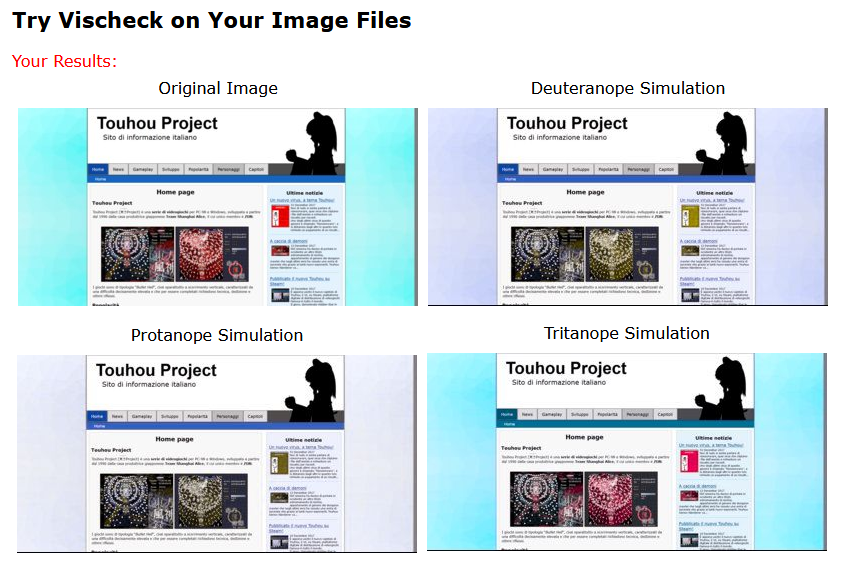
\includegraphics[width=0.8\linewidth]{images/daltonismo}
				\caption{Risultati ottenuti su Vischeck}
			\end{figure}
			Ulteriormente anche su mobile sono state testata le stesse varianti di colorazione agendo sulle impostazioni di sviluppo di Android 7.1 presenti sulla rom MIUI versione China Dev, purtroppo gli screenshots effettuati in questa modalità di colore apparivano senza filtro, e per questo motivo non è stato possibile riportare i test effettuati in questo documento.
			
			\subsection{VEGA}
			\`{E} stato utilizzato lo strumento VEGA scaricabile gratuitamente da \url{subgraph.com/vega} per controllare eventuali errori di sicurezza all'interno del sito.\\
			
			\begin{figure}[H]
				\centering
				\includegraphics[width=0.8\linewidth]{images/VEGA}
				\caption{Risultati ottenuti su VEGA}
			\end{figure}
			Dopo alcune correzioni apportate sono rimaste presenti delle problematiche, ma sono dettate dalla configurazione attuale di XAMPP configurato per essere utilizzato in un ambiente di sviluppo e non di produzione.

		\section{Test su diversi dispositivi}
			Il sito è stato testato su varie macchine e sistemi operativi. Nelle sezioni seguenti verranno elencati assieme ai browser e alle risoluzioni testate.
				\subsection{Windows 10}
				Sono state testate le risoluzioni di 1080p e 2160p con i browsers:
				\begin{itemize}
					\item Chromium 64
					\item Google Chrome
					\item Edge
					\item Internet Explorer 11
					\item Firefox Quantum
					\item Waterfox 57
					\item Firefox Nightly 60a1
					\item Mozilla Firefox 3
					\item Netscape 7
				\end{itemize}
				Si è notato che Mozilla Firefox 3 utilizza una dimensione errata dell'immagine nella testata. Questo aspetto rovina leggermente il rendimento grafico ma non ne compromette le funzionalità, in quanto tutti i contenuti risultano perfettamente fruibili dall'utente.\\
				Un Secondo appunto riguardante Firefox 3 è l'incompatibilità con parte del codice JavaScript: solamente il controllo della compilazione dei campi di testo funziona correttamente.\\
				Internet Explorer 11, con la modalità Explorer 9, non genera nessun problema, ed anche il problema della dimensione della testata riscontrato su Firefox 3 è assente.\\
				Internet Explorer 5, 7 ed 8 non supportano il MIME xhtml+xml, quindi il sito non viene visualizzato ma ne viene proposto il download. Nel caso venga incorrettamente settato il MIME html allora il sito funziona perfettamente sulla versione 7 ed 8 del browser, compresa la visualizzazione del tag Ruby. In questo caso alcune funzionalità JavaScript ed alcune proprietà CSS non vengono riconosciute ma questo non compromette l'utilizzo del sito.\\ 
				Con Microsoft Edge 16 (ultima versione) non sono stati riscontrati problemi. \\
				Non sono stati rilevati ulteriori problemi o incompatibilità con i browser sopra menzionati ad esclusione di Netscape, anche variando la grandezza del font, dello zoom della pagina, della dimensione della finestra e disattivando JavaScript.\\
				Il sito è stato provato anche su Netscape 7, soprattutto per soddisfare una curiosità personale e per comprendere meglio l'evoluzione dello sviluppo dei siti web negli anni. Il risultato è ovviamente insoddisfacente, i tag div e p sono visualizzati erroneamente, moltissime proprietà css non sono correttamente riconosciute dal browser e soprattutto le mediaquery non sono supportate, facendo caricare al sito la versione mobile.\\
				Ovviamente non sono stati presi provvedimenti per migliorare la situazione con Netscape, in quanto il software è datato al 2002 e non è più in uso in nessun ambito.
				
				\subsection{GNU/Linux Fedora 27}
				Sono state testate le risoluzioni di 1800p e 2160p con i browsers:
				\begin{itemize}
					\item Firefox Quantum
					\item Google Chrome
					\item Firefox 56
					\item Lynx
				\end{itemize}
				Durante la fase di test su questa piattaforma non sono emerse problematiche a livello di compatibilità o visibilità nonstante le alte risoluzioni. Inoltre su questa piattaforma è stata testata la leggibilità del sito con l'utilizzo del browser cli Lynx.

				\subsection{MacOS High Sierra}
				Sono state testate le risoluzioni di 1800p, 2160p e 2880x1800p con i browsers:
				\begin{itemize}
					\item Safari 11.0.2
					\item Firefox Quantum
					\item Google Chrome
				\end{itemize}
				Durante la fase di test su piattaforma MacOS non è emersa alcuna problematica per quanto riguarda visibilità e compatibilità. Il sito viene visualizzato correttamente in tutti e tre i browser provati, nonostante le alte risoluzioni dei display utilizzati.

				\subsection{FreeBSD 11}
				\`{E} stata testata la risoluzione 1080p sui seguenti browsers:
				\begin{itemize}
					\item Firefox Quantum
					\item Lynx
					\item Lynx da CLI
				\end{itemize}
				Il sito è stato testato con il browser Lynx utilizzando la console senza x11 o Wayland, quindi da terminale/CLI, e con x11, quindi da una finestra di emulazione del terminale di dimensione variabile.\\
				In entrambi i casi il contenuto era fruibile.

				\subsection{Dispositivi mobili}
				Di seguito sono elencati i vari dispositivi mobili sui quali il sito è stato testato
				\begin{itemize}
				\item Xiaomi Redmi 4X (Chinese Dev) con Miui browser, Firefox Rocket e Waterfox con una risoluzione di 720p
				\item Amazon Kindle Touch 2 (7' generazione) con schermo e-ink in bianco e nero, con una risoluzione di 800x600 e con il browser sperimentale fornito di default.
        		\item Testato su Ipad Pro 10.5' su browser Safari versione 11.2.5 con una risoluzione di 2224x1668 
				\end{itemize}
			
				In tutti i dispositivi testati il sito si adatta perfettamente alla risoluzione dello schermo e non sono presenti problemi di compatibilità, neppure con JavaScript.\\
				L'unico appunto da fare è la mancanza di supporto degli RSS, che vengono letti come file di testo normali, ad eccezione di Waterfox che invece ne propone il download.\\
				Anche su schermo e-ink in bianco e nero i link rimangono sufficientemente marcati rispetto al resto del testo e tutte le sezioni rimangono distinguibili.
			
				\begin{figure}[H]
					\centering
					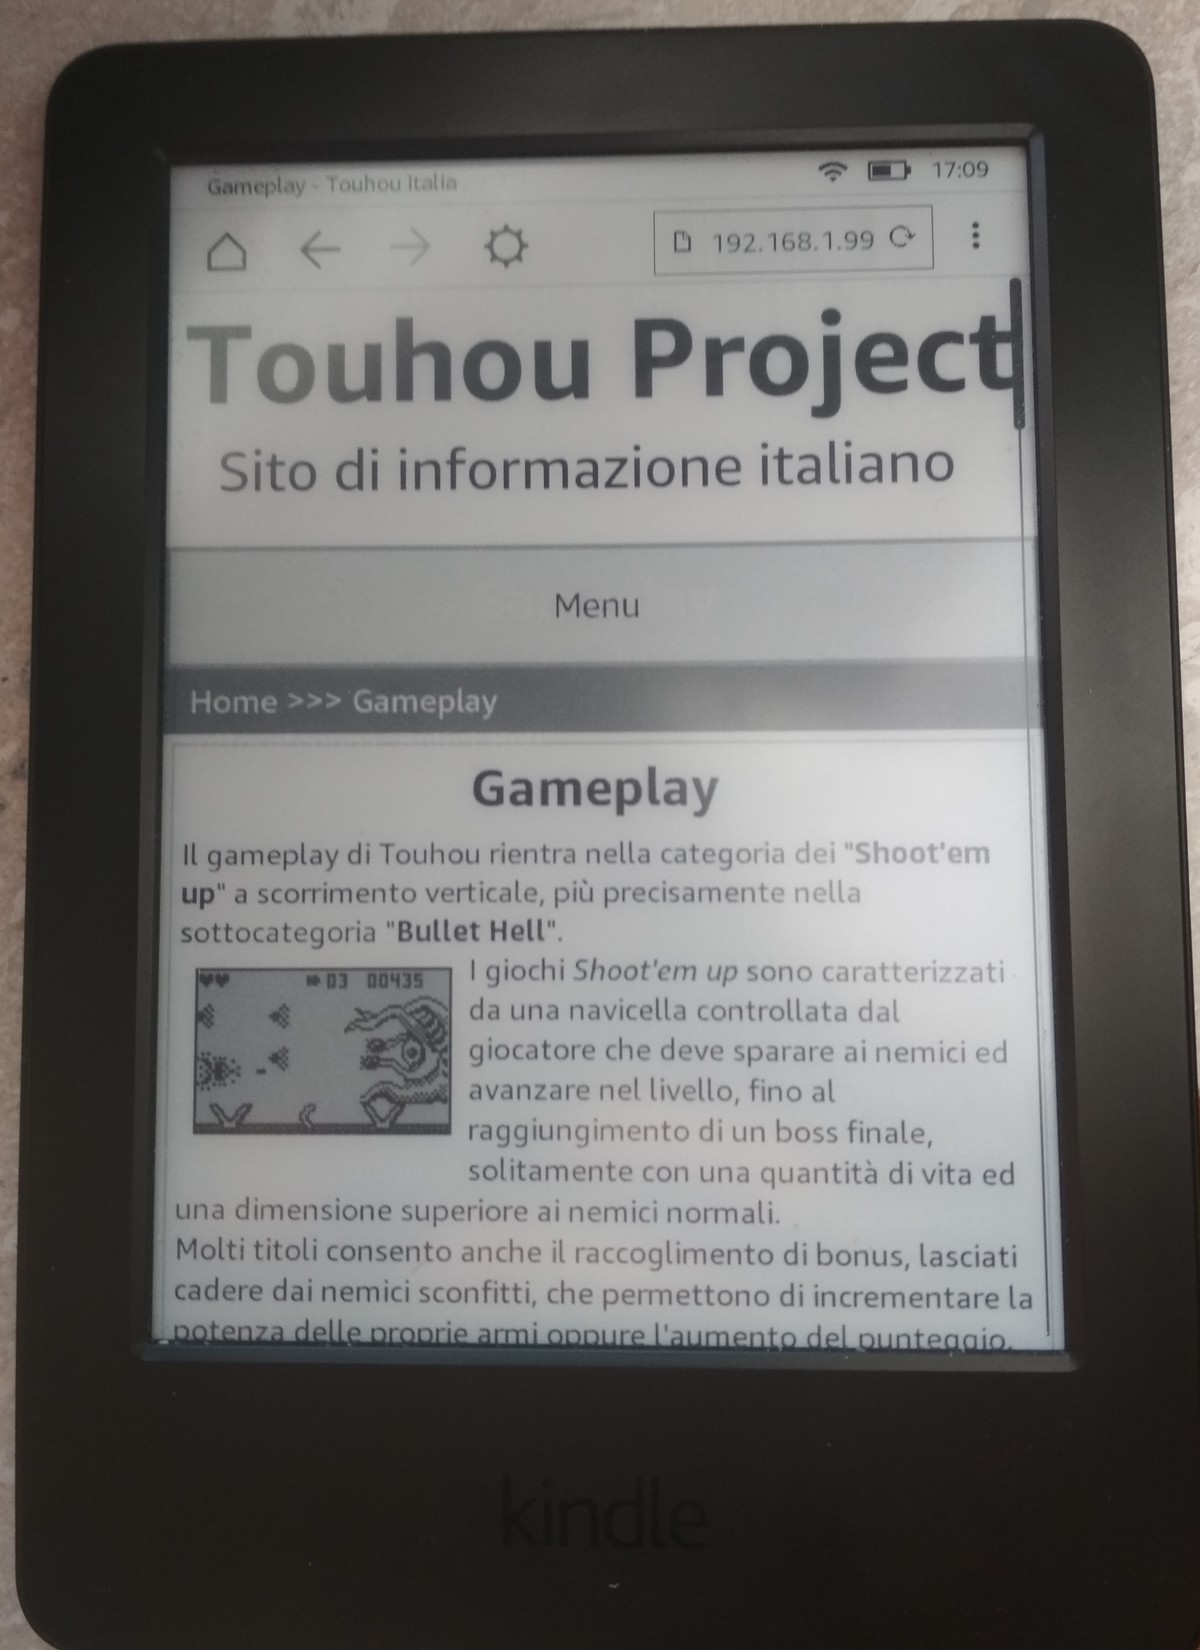
\includegraphics[width=0.7\linewidth]{images/Kindle}
					\caption{Il sito web sul dispositivo Amazon Kindle Touch 2}
				\end{figure}
			
		\section{Test con diverse impostazioni utente}
			Il sito è stato testato con multiple impostazioni utente, come citato nella sezione riguardante le piattaforme di testing sono state testate risoluzioni che vanno dall 600p al 2160p senza presentare problemi di visualizzazione. Oltre al test per le varie risoluzioni e dispositivi si è testata la visualizzazione del sito con dimensioni del testo di che vanno 16pt a 44pt e con uno zoom elevato mantenendo comunque una buona fruibilità del sito.\\
			\`{E} stata presa in considerazione anche la possibilità che un utente abbia bloccato, oppure non abbia la possibilita se pur remota di non poter eseguire Javascript, e nonostante questo il sito rimane comunque egualmente navigabile in tutte le sue parti, senza far trasparire in modo palese la mancanza di Javascript.\\

		\section{Lynx e come potrebbe essere se letto}
			Il sito è stato testato con il browser Lynx, nonostante la visualizzazione solo testuale il sito rimane comunque navigabile seppur non in modo agevole se non si è abituati al utilizzo dei browser testuali.
			\begin{figure}[H]
				\centering
				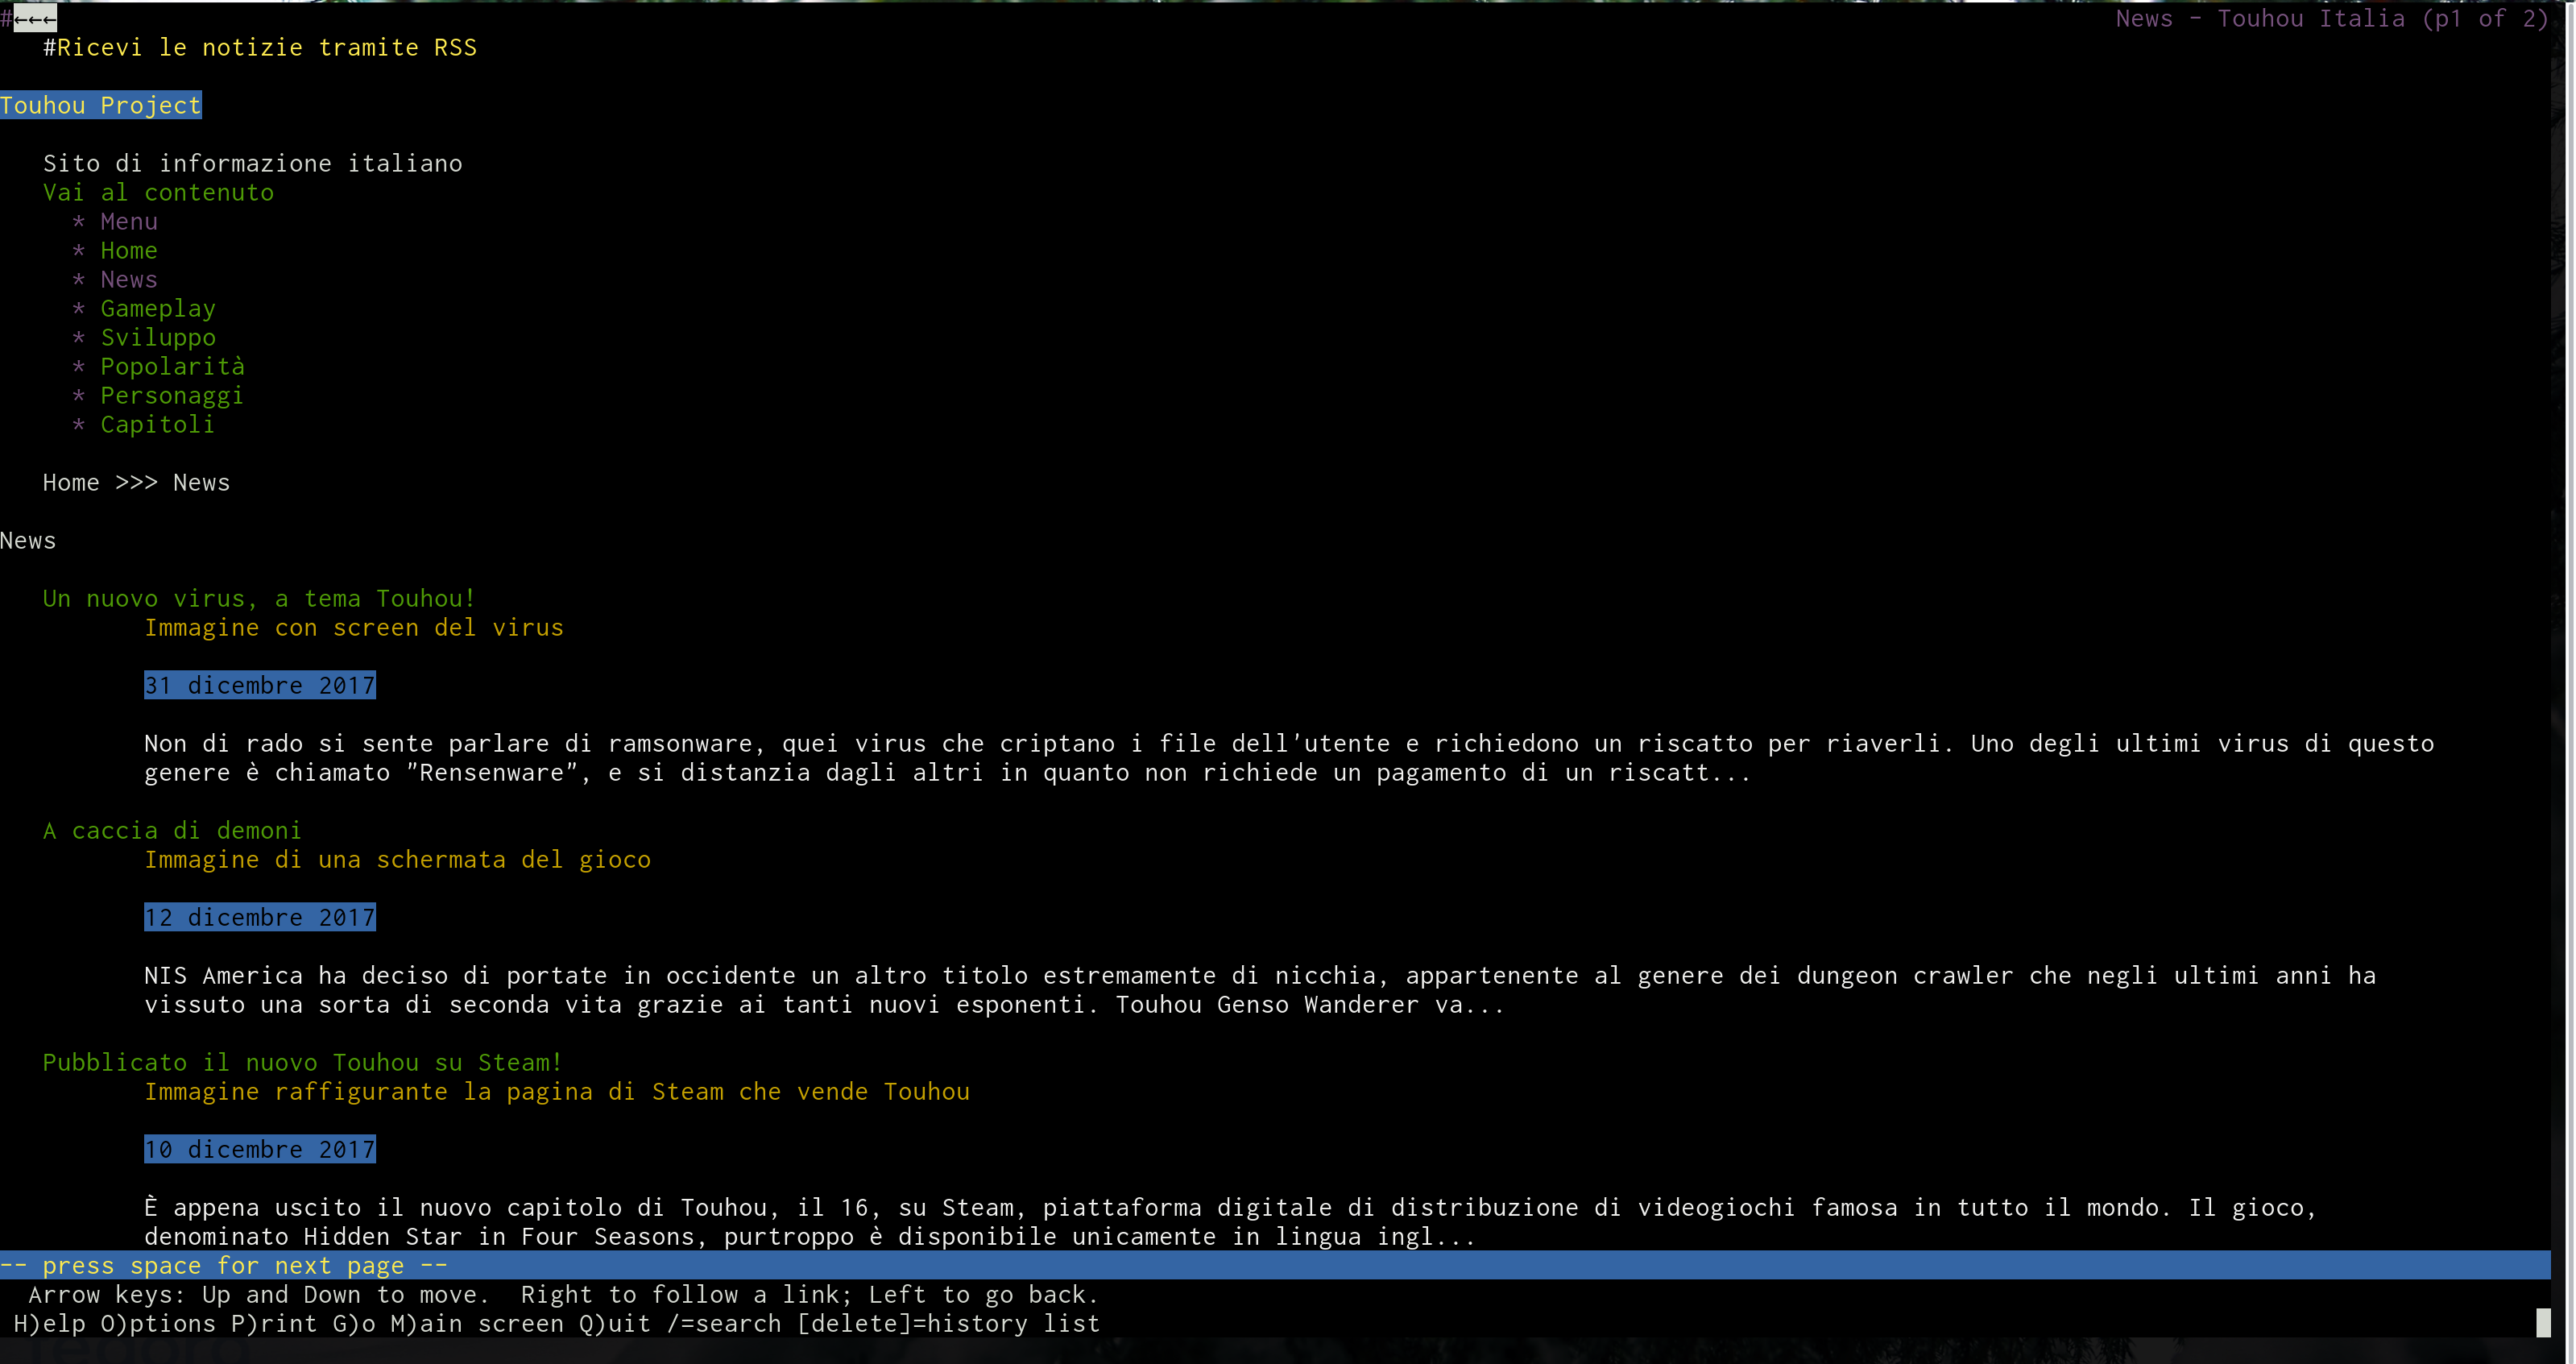
\includegraphics[width=1.2\linewidth]{images/Lynx2}
				\caption{Esempio di pagina del sito web su Lynx}
			\end{figure}
		

	\chapter{Ambiguità incontrate e scelte intraprese}
		\section{Descrizione della sessione}
			In questa sezione del documento sono elencate tutte le decisioni prese su aspetti ambigui presenti nel sito\\
		\section{Utilizzo della lingua straniera}
			\subsection{Furigana}
				A supporto dei termini scritti in kanji, sono stati inseriti i furigana, cioè la pronuncia del termine in caratteri hiragana (pratica comune in siti che presentano termini giapponesi mirati ad adolescenti o a stranieri che potrebbero avere una discreta conoscenza del giapponese).\\
				Questo avviene anche in Giappone in quanto i kanji essendo molteplici (si calcola circa 18'000) è frequente che i lettori ne trovino di sconosciuti e si cerca di aiutarli inserendo a lato la pronuncia nel sillabario utilizzato per i termini giapponesi, cioè l'hiragana.\\
				A volte, se il termine è di origine straniera, il furigana potrebbe presentarsi con caratteri del sillabario katanaka. Questo avviene di rado e non è presente nel nostro sito, in quanto preferiamo presentare le parole inglesi direttamente in alfabeto latino.
			\subsection{Traslitterazioni}
				Le traslitterazioni dalla lingua giapponese sono spesso imprecise e ci sono controversie sulla pronuncia persino nella stessa lingua giapponese; quindi si è scelto, in caso di screen reader, di lasciare leggere le parole traslitterate usando l'alfabeto italiano, che si rivela in molti casi anche più preciso rispetto all'inglese nella lettura dei termini.\\
				Alcune parole giapponesi, che si rivelano essere lette più fedelmente dalla pronuncia inglese, sono state marcate come tali.\\
				Successivamente c'è anche da considerare che alcuni termini sono pronunciati erroneamente per avvicinarli di più a pronunce occidentali, la stessa parola Touhou dovrebbe essere letta come Tōhō, o Tohō, ma la pronuncia americana e successivamente europea è stata resa Touhou.\\
				Se le parole traslitterate fossero state marcate come lingua giapponese i termini sarebbero stati considerati in alfabeto "romaji" (romano, cioè l'alfabeto latino), e quindi traslitterati nuovamente in katakana per poi essere letti usando la lingua giapponese, che avrebbe portato a pronunce ancora più errate, in quanto non c'è una corrispondenza precisa tra l'alfabeto e il sillabario.
				
			\subsection{Termini errati}
				Nel sito appaiono termini con delle lettere maiuscole poste senza rispettare la grammatica inglese. In quei casi si è trascritto il termine esattamente come appare nella documentazione ufficiale, all'interno del videogioco o nei file dello stesso. Alcuni esempi sono "Nights of Night" o "U.N. Owen Was Her". In questo ultimo caso non ci è dato sapere cosa significhi U.N., si pensa possa essere un riferimento a Una Nancy Owen, ma non essendoci alcuna conferma ufficiale è stato preferito ometterlo.\\

	\chapter{Funzionalit\`{a} desiderabili}
		\section{Descrizione della sezione}
		Nella seguente sezione verranno illustrate le funzionalità che nel caso di un progetto reale verrebbero inseriti ma che in questo caso non sono stati inclusi vista l'eccessiva complessita di alcuni rapportata allo scopo e al tempo previsto per questo progetto.

		\section{Pagine social network di supporto al sito}
		Nella maggior parte dei siti moderni è presente un qualche collegamento a pagina nei social network, nel nostro caso non è stata ritenito un impiego di tempo produttivo per gli scopi del progetto andare a creare queste pagine social visto che poi si sarebbe trattato di inserire i link a queste nel sito, nel nostro caso sarebbero stati inseriti nella sidebar assieme ai feed rss.

		\section{Editor HTML per gli amministratori}
		La possibilità della realizzazione di un editor HTML come quelli presenti all'interno dei CMS è stata esclusa visto il tempo che sarebbe stato necessario per realizzarlo che sarebbe stato eccessivo. Comunque nonstante non sia stato sviluppato si ritiene che l'implementazione di un editor di questo per la parte di amministrazione renderebbe molto più efficace la gestione delle funzionalità che richiedono di manipolare testo che poi verra inserito nel database come blocchi di codice html.   
		
		\section{Image picker}
		Una ultima funzione avanzata che migliorerebbe l'utilizzo del sito da parte dell'amministratore, che si collega all'editor HTML, sarebbe quella di poter selezionare una immagine da inserire in un articolo direttamente dalla galleria delle immagini, o caricarla al momento all'interno della galleria, senza la necessità di spostarsi sulla sezione immagini, caricarla, copiare il link, tornare alla notizia che stava inserendo e compilando il tag html per l'inserimento dell'immagine.



	\chapter{Suddivisione del lavoro}
	\section{Suddivisione per membro del gruppo}
	\subsection{Bisello Samuele - Matricola 1122438}
	\begin{itemize}
		\item Scrittura contenuti per la pagina capitoli
		\item Definizione stile del login e di svariati elementi, soprattutto nella parte di amministrazione
		\item Script JS per la validazione delle form lato admin
		\item Raffinamento e verifica delle form
		\item Inserimento dello sticky header
		\item Test su MacOS High Sierra e iOS
		\item Sviluppo di una parte di codice PHP per la connessione con il database
	\end{itemize}
	\subsection{Cailotto Mirco - Matricola 1123521}
	\begin{itemize}
		\item Creazione struttura base del sito
		\item Raccolta e stesura nella relazione di tutti gli aspetti relativi alla lingua giapponese
		\item Raccolta di riferimenti per il contenuto del sito
		\item Scrittura contenuti per pagina di home page, gameplay, realizzazione, popolarità
		\item Creazione php per le news e svariate pagine di amministrazione
		\item Creazione bozza dello stile per le pagine utente e amministrazione
		\item Scrittura della funzione php per l'upload delle immagini
		\item Scrittura del sistema di errori in PHP forniti all'utente
		\item Creazione della struttura del database
		\item Controllo dei valori inseriti all'interno del database
		\item Parsing degli input per evitare SQLInjection
		\item Svolgimento di test automatici
		\item Stesura dello scheletro della relazione
		\item Stesura parte abstract, di analisi dell'utenza e di ambiguità linguistica della relazione
		\item Creazione dello script per lo zoom delle immagini
		\item Raffinamento dello sticky header
		\item Test su sistema Windows e Android
		\item Creazione RSS
	\end{itemize}
	\subsection{Todescato Matteo - Matricola 1121857}
	\begin{itemize}
		\item Scrittura contenuti per la pagina dei personaggi
		\item Gestione degli amministratori nella parte PHP e relativa parte del database
		\item Stesura del login
		\item Definizione dello stile grafico adottato
		\item Creazione dello sfondo
		\item Script JS per la validazione delle form lato utente
		\item Inserimento notizie
		\item Test su sistema Linux
		\item Stesura della parte di realizzazione della relazione
	\end{itemize}

\end{document}
